\section{Parsing math expressions}
\label{sec:parsing_math_expressions}

\begin{frame}
	\frametitle{Parsing math}
	\framesubtitle{XKCD Dimensional Analysis: \url{https://xkcd.com/687/}}
	\begin{center}
		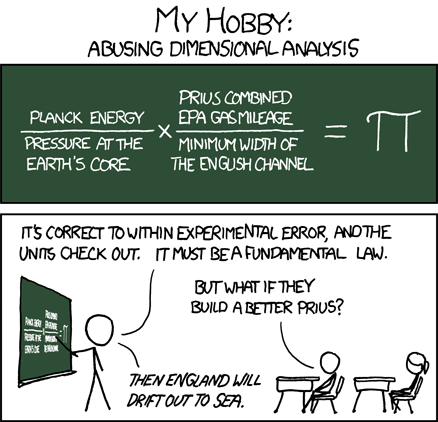
\includegraphics[width=0.5\textwidth]{figures/math.png}\\
	\end{center}
\end{frame}

\begin{frame}
	\frametitle{Parsing math}
	
	\begin{problemblock}{Back to primary school}
		Given a math expression containing:
		\begin{itemize}
			\item Numbers
			\item Parentheses
			\item Unary operators: $-$ and $\sqrt{\invisible{x}}$
			\item Binary operators: $+$, $-$, $/$, and $\times$
		\end{itemize}
		What number does the expression evaluate to?
	\end{problemblock}
	\pause
	\begin{questionblock}{A simple example}
		$((8-\sqrt{16})\times 2) / (-4 + 3)$
		\vspace{-10pt}
		\begin{multicols}{2}
		\begin{enumerate}[A.]
			\item -8
			\item -4
			\item 4
			\item 8
			\item Ummmmmmm\dots
		\end{enumerate}
		\end{multicols}
	\end{questionblock}
\end{frame}

\begin{frame}
	\frametitle{A parse tree}
	\begin{questionblock}{A simple example}
		$((8-\sqrt{16})\times 2) / (-4 + 3)$
	\end{questionblock}
	\pause
			
	\begin{answerblock}{The parsing tree}
	\begin{columns}
		\column{0.555\textwidth}
  \begin{tikzpicture}[
    level distance = 2.5em,
    level 1/.style={sibling distance=11em},
    level 2/.style={sibling distance=4.5em},
    level 3/.style={sibling distance=2.25em},
  ]
  \node[ellipse] (t1) {/}
    child { node[ellipse] {$\times$}
      child { node[ellipse] {-} 
				child { node[ellipse] {8}} 
				child { node[ellipse] {$\sqrt{\invisible{x}}$}
					child { node[ellipse] {16}}}}
			child { node[ellipse] {2}}}
    child { node[ellipse] {+}
			child { node[ellipse] {-}
				child { node[ellipse] {4}}}
			child { node[ellipse] {3}}};
  \end{tikzpicture}\\
		\column{0.355\textwidth}
		\begin{itemize}
			\item This tree represents the expression.
				\pause
			\item By parsing this tree, we can parse the expression.
		\end{itemize}
	\end{columns}
	\end{answerblock}
\end{frame}

